% --------------------------------------------------------------
% This is all preamble stuff that you don't have to worry about.
% Head down to where it says "Start here"
% --------------------------------------------------------------
 
\documentclass[12pt]{article}
 
\usepackage[margin=1in]{geometry} 
\usepackage{amsmath,amsthm,amssymb}
\usepackage[pdftex]{graphicx}
\usepackage{parskip}
\usepackage{hyperref}
\usepackage[all]{hypcap}
\usepackage{amsmath}
\usepackage{amsfonts}
\usepackage{enumitem}
\usepackage{amsmath}
\usepackage{amssymb}
\usepackage{graphicx}
\usepackage[colorinlistoftodos]{todonotes}
\usepackage{tikz}
\usepackage{gensymb}
\usepackage{mathtools}
\usepackage{framed}

\newcommand\Circle[1]{%
  \tikz[baseline=(char.base)]\node[circle,draw,inner sep=2pt] (char) {#1};}

\newcommand\tikzmark[2]{
  \tikz[remember picture, overlay]\node[inner sep=0pt] (#1) {#2};}

 
\newcommand{\N}{\mathbb{N}}
\newcommand{\Z}{\mathbb{Z}}

\newcommand\Myperm[2][^n]{\prescript{#1\mkern-2.5mu}{}P_{#2}}
\newcommand\Mycomb[2][^n]{\prescript{#1\mkern-0.5mu}{}C_{#2}}
 
\newenvironment{theorem}[2][Theorem]{\begin{trivlist}
\item[\hskip \labelsep {\bfseries #1}\hskip \labelsep {\bfseries #2.}]}{\end{trivlist}}
\newenvironment{lemma}[2][Lemma]{\begin{trivlist}
\item[\hskip \labelsep {\bfseries #1}\hskip \labelsep {\bfseries #2.}]}{\end{trivlist}}
\newenvironment{exercise}[2][Exercise]{\begin{trivlist}
\item[\hskip \labelsep {\bfseries #1}\hskip \labelsep {\bfseries #2.}]}{\end{trivlist}}
\newenvironment{reflection}[2][Reflection]{\begin{trivlist}
\item[\hskip \labelsep {\bfseries #1}\hskip \labelsep {\bfseries #2.}]}{\end{trivlist}}
\newenvironment{proposition}[2][Proposition]{\begin{trivlist}
\item[\hskip \labelsep {\bfseries #1}\hskip \labelsep {\bfseries #2.}]}{\end{trivlist}}
\newenvironment{corollary}[2][Corollary]{\begin{trivlist}
\item[\hskip \labelsep {\bfseries #1}\hskip \labelsep {\bfseries #2.}]}{\end{trivlist}}
 
 
% --------------------------------------------------------------
%                         Start here
% --------------------------------------------------------------
 
%\renewcommand{\qedsymbol}{\filledbox}
 
%%\title{Assignment 1}%replace X with the appropriate number
%%\author{Muhammad Haris (mh02272)\\ %replace with your name
%%MATH 205 - Linear Algebra} %if necessary, replace with your course title

\newcommand{\mat}[1]{\boldsymbol { \mathsf{#1}} }
 
\begin{document}
\setlength{\parskip}{10pt} % 1ex plus 0.5ex minus 0.2ex}
\setlength{\parindent}{0pt}
\DeclareGraphicsExtensions{.pdf,.png,.gif,.jpg}
%\maketitle

\begin{titlepage}

\newcommand{\HRule}{\rule{\linewidth}{0.5mm}} % Defines a new command for the horizontal lines, change thickness here

\center % Center everything on the page
 
%----------------------------------------------------------------------------------------
%	HEADING SECTIONS
%----------------------------------------------------------------------------------------

\textsc{\LARGE Habib University}\\[1.5cm] % Name of your university/college
\textsc{\Large EE 322L - Analog and Digital Communication}\\[0.5cm] % Major heading such as course name
%\textsc{\large Assignment 1}\\[0.5cm] % Minor heading such as course title

%----------------------------------------------------------------------------------------
%	TITLE SECTION
%----------------------------------------------------------------------------------------

\HRule \\[0.4cm]
{ \huge \bfseries \textsc{Demonstrating Scheduling Algorithms} }\\[0.4cm] % Title of your document
{ \large \bfseries \textsc{Lab Project Report} }\\[0.4cm] 
\HRule \\[1.5cm]
 
%----------------------------------------------------------------------------------------
%	AUTHOR SECTION
%----------------------------------------------------------------------------------------
\begin{minipage}{0.4\textwidth}
\begin{flushleft} \large
\emph{Group Members:}\\
Syed Sameer Nadeem (sn02902)\\
Muhammaed Haris (mh02272)\\
\emph{Section:}
L2\\
\end{flushleft}
\end{minipage}
~
\begin{minipage}{0.4\textwidth}
\begin{flushright} \large
\emph{Instructor:} \\
Sir Tariq Mumtaz \\
Ma'am Zareen Tabssum\\
Sir Muhammad Raza Rizvi
% Supervisor's Name
\end{flushright}
\end{minipage}\\[2cm]

% If you don't want a supervisor, uncomment the two lines below and remove the section above
%\Large \emph{Author:}\\
%John \textsc{Smith}\\[3cm] % Your name

%----------------------------------------------------------------------------------------
%	DATE SECTION
%----------------------------------------------------------------------------------------

{\large \today}\\[2cm] % Date, change the \today to a set date if you want to be precise

%----------------------------------------------------------------------------------------
%	LOGO SECTION
%----------------------------------------------------------------------------------------

%\includegraphics{logo.png}\\[1cm] % Include a department/university logo - this will require the graphicx package
 
%----------------------------------------------------------------------------------------

\vfill % Fill the rest of the page with whitespace

 \newpage
 
 \tableofcontents
 
 \newpage

\end{titlepage}

 

 
 \newpage
 
 \section{Abstract}
 
The aim of this project was to demonstrate scheduling algorithm after synchronizing nodes in an Ad-Hoc network for pair to pair communication. The need for scheduling arises due to the fact that the spectrum is limited and in order to cater to more users, the users are scheduled such that their messages do not interfere with each other. Arduino-RF module pairs were used to demonstrate nodes in an Ad-Hoc network and each node was assigned individual slots for receiving and transmitting. The first part was to synchronize, where one of the nodes triggers a signal and then the rest wait till they recieve the trigger. Then the actual communication starts. However since the channel is not perfect the trigger is sent multiple times whihc in turn creates discrepancies and does not allow perfect synchronization. However, the communication goes fine if the channel is satisfactory and the scheduling is demonstrated. 
 
 \section{Introduction}
 
 Wireless communication is an integral part of our daily lives. Unlike wired communication where the channel or medium of the is wire/fiber-optics, wireless communication relies on air as its medium. Although having air as the medium saves cost on laying cables, however the spectrum in which the messages are modulated and transmitted is quite limited and expensive. There are tonnes of techniques to increase the throughput capacity. One of the techniques is to divide in time, and schedule effectively in such a way that the same spectrum (of 433 MHz carrier in this case) is shared by all but not all the time but rather each user is given a slot to receive and transmit.
 
 The project makes use of pair-to-pair communication instead of a centralized network. Pair-to-pair network or Ad-hoc network doesn't rely on a centralized Base Station to schedule. In this system the individual nodes schedule themselves and synchronize on their own rather than having a single clock being fed to the Base Stations. This adds up to the challenge of locally synchronizing the nodes. 
 
 \section{Rationale of the Solution}
 
 The limited nature of the spectrum makes us to use it more efficiently in such a way that more number of users can be incorporated. It is to ensure that the throughput capacity of the system is increased. An algorithm is devised to synchronize the nodes first. And then each node is assigned a slot, $x$ seconds, in time every $T$ seconds. The lesser is $x$ the better the system and lower is the latency. However for demonstration purposes $x=2$ seconds is this case. 
 
 The solution partially takes care of the issue of security breach as well. If a node tries to receive data when it is not its time then the node can't interpret the data is ciphered such that the node won't be able to make sense of the data it receives even if it tries to intercept the data. As of yet we haven't incorporated the idea of ciphering but rather we have made it in such a way that for example node 1 has to receive specific bits in a specific slot if it recieves something else then the LED won't blink. 
 
 \section{Discussion}
 
The approach taken to form an algorithm is to synchronize the nodes first. That is a trigger signal sent by the first node and the the rest of the two nodes stay silent until they recieve the trigger node and then they start the communication procedure. The following is the code for the syncronisation,

\begin{figure}[h]
\centering
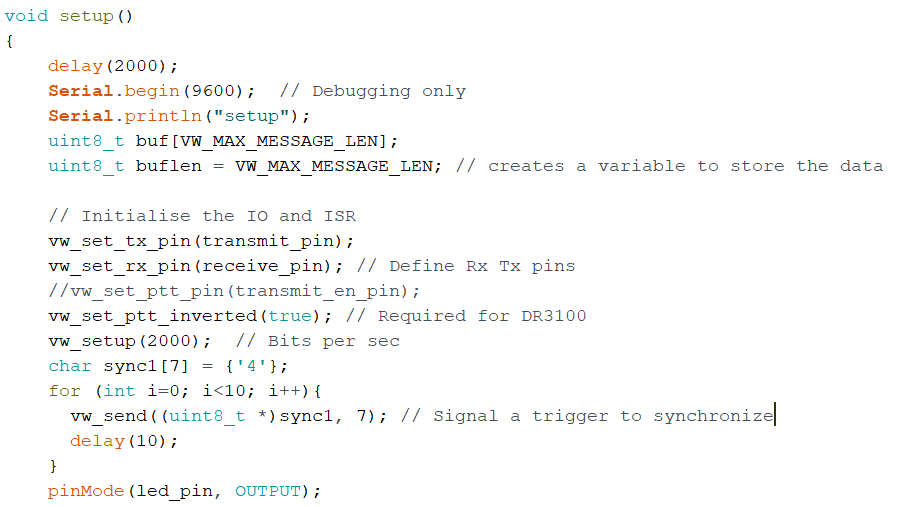
\includegraphics[scale=0.5]{sync1.PNG}
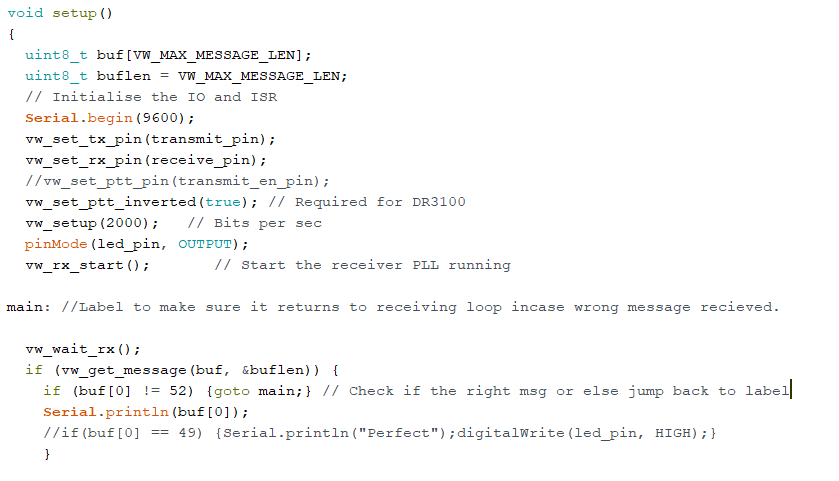
\includegraphics[scale=0.5]{sync2.PNG}
\caption{Code for (a) Node 1 triggers a signal (b) Node 2 and 3 wait till they recieve the right message}
\end{figure}


 Then comes the part where the nodes communicate with each other the following are the slots for each of the nodes recieving and transmitting,
 
\begin{center}
\begin{tabular}{ |c|c|c| } 
 \hline
 Node & Transmit (s) & Recieve (s) \\ 
 \hline
 \hline
 1 & 0-2 & 2-4, 4-6 \\ 
 2 & 2-4 & 0-2, 4-6 \\ 
 3 & 4-6 & 0-2, 2-4 \\ 
 \hline
\end{tabular}
\end{center}

As mentioned above the slots can be made smaller and the communication can be made more smooth but the problem lies in the fact that this project is to demonstrate and the synchronization is not perfect so the slots are of 2 seconds each. Ideally they should be as short as possible. The following is the example code for the the schedulling (replicated for the other nodes),
\newpage

 \begin{figure}[h]
 \centering
 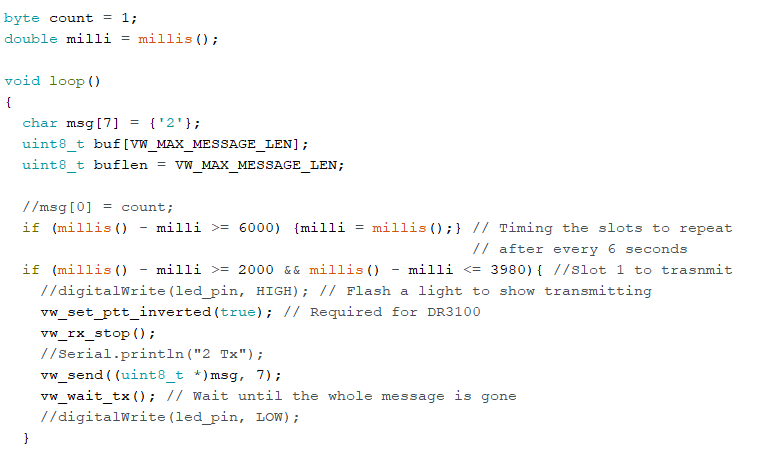
\includegraphics[scale = 0.4]{algo1.PNG}
  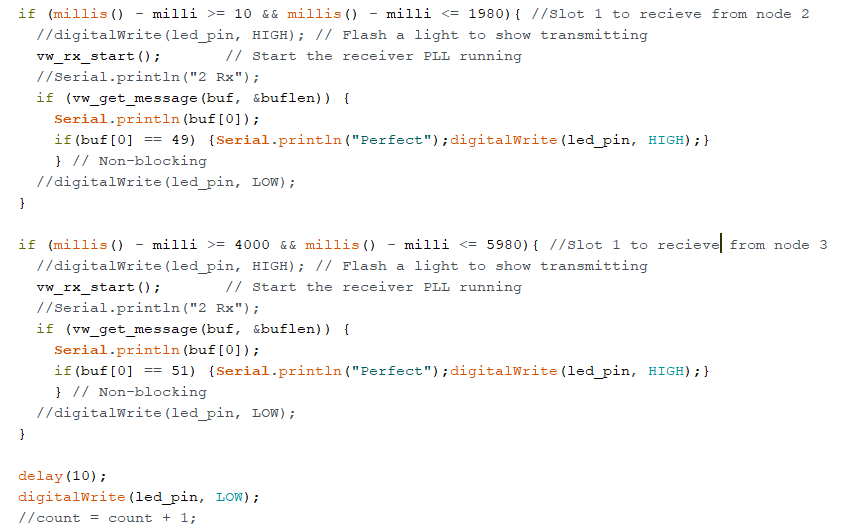
\includegraphics[scale = 0.5]{algo2.PNG}
 \caption{Code for the scheduling algorithm}
 \end{figure}
 
 Notice also the guard band we have left in time slots of nearly 10 ms. This gaurd band is ideally in the order of nano seconds and is left to ensure multipaths do not reach however here it is left since the nodes are not perfectly synchronized. 

\section{Circuit Diagram}
 
 The following is the circuit diagram of one such node. The same circuit is replicated for each node.  
 
 \begin{figure}[h]
 \centering
 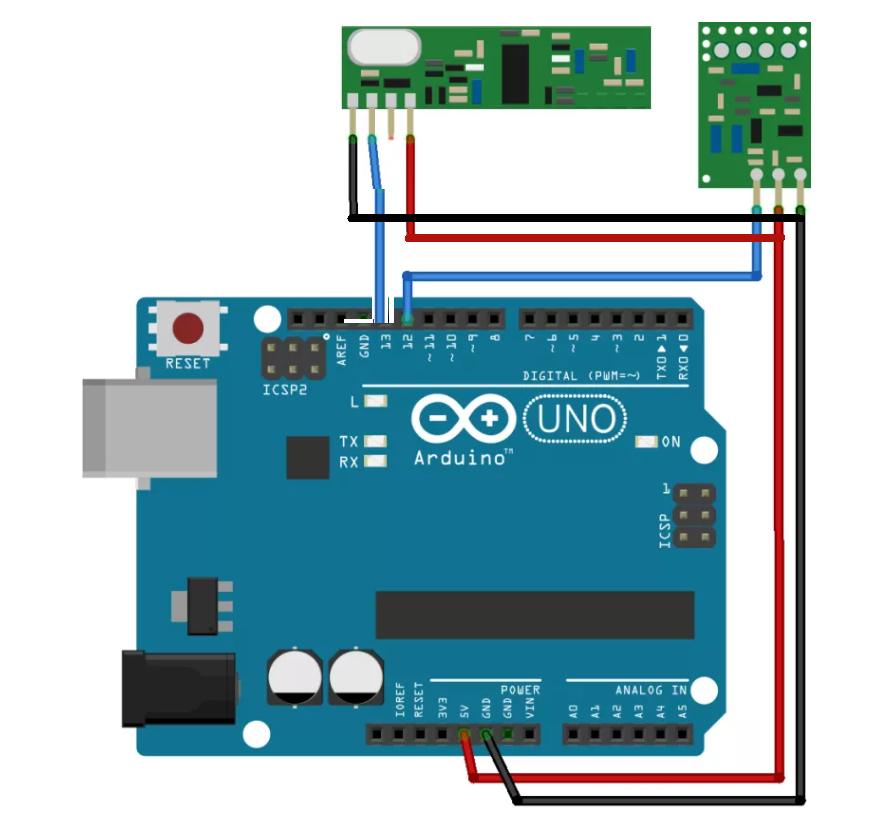
\includegraphics[scale = 0.35]{circuit1.PNG}
 \caption{Circuit Diagram of the nodes of the Solution presented}
 \end{figure}
 

\section{Choice of Material}

 The following items were,
 
 \begin{itemize}
 \item Arduinos
 \item RF Modules Pairs, 433 MHz
 \item Connectors
 \end{itemize}
 
 Arduino paired with 433 MHz RF modules provide a very cheap base for demonstrating any sort of scheduling algorithm. There exist expensive alternatives as well where the module has built-in transmitter and receiver within the same module and it is easy to code since the entire interrupt service routine is not required to be defined but these items are cost effective. We have used built-in LEDs for the Arduinos. 

\section{Conclusions and Future Recommendations}

The project overall went fine except for a few improvements that coul be made. Initially we were using radio head library but that did not give us freedom to use both the transmitter and the reciever on the same arduino since once the transmitter transmits it needs to be manually disabled or else it wont allow the reciever to work using some ISR. However then we used virtual wire library which gives us flexibility to enable and disable the transmitter manually although increases the length of the code. 

Another feature that could be added is the acknowledgement protocol where the nodes send an acknowledgement after recieving the message. This would ensure data is not lost if acknowledgement is not sent then actions may be taken to investigate the breach. 

Another improvement would be to cipher the message before sending them. Right now we have just programmed the LED not to blink if the message sent is not the right one with regard to the slot. But in future in order to prevent the breach a method could be to cipher at the transmitter and decode using pseudo random key at the reciever. 

The project successfully demonstrated scheduling algorithms in an Ad-Hoc network. 

% --------------------------------------------------------------
%     You don't have to mess with anything below this line.
% --------------------------------------------------------------
 
\end{document}